\subsection{Questionnaire:}

\begin{enumerate}
\item {\bfseries\itshape What value of $q$ returns {\bfseries\itshape Partition} when all the elements in array $A [p, ..., r]$ have the same value ?}\hfill 

When we take a look to the algorithm we can see that if the element has the same value or the value is lower than the pivot, the algorithm exchange the positions in the array, first the element in position $A[j]$ is changed by the element which is in the position $A[q]$ then,  $q$ is moving up at the same time of $j$ which is the index of the elements bigger than pivot, so when it is finished the first time the $q$ has the same value as r (value of position or pivot), in that first case $r$ is equal to $n$, where $n$ is the size of the array is  {\bfseries\itshape n - 1}, and the quicksort is called once again, for this time the $q$ equal {\bfseries\itshape n - 2}, the next time $q$ equal {\bfseries\itshape n - 3} and so on, this is one of the worst cases in this algorithm, because is always doing the merge n times in place of $T(\ \frac{n}{2}\ )$. This procedure it's represented in Figure 5.1.0.

\begin{figure}[H]
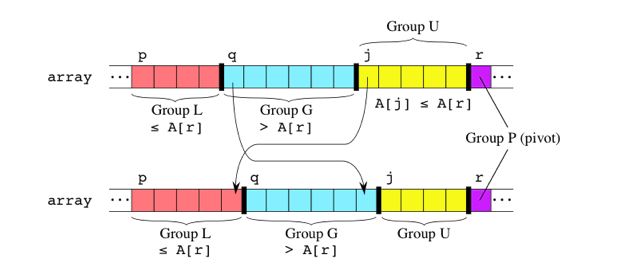
\includegraphics[scale=.6]{quicksort}
\centering \linebreak \linebreak Figure 5.1.0: Array partition. 
\end{figure}

In the image above is illustrated the previous procedure, in this case the group G is always 0 because there are not number greater than the pivot, when the index j reaches the value index of pivot, the q takes the same value, so if the $n$ equal $10$ where $n$ is the number of elements, the first time $q$ is 9 because the position of the element $A[10]$ is $9$, then $8$, then $7$ and so on. \hfill \break

 {\bfseries\itshape\color{armygreen}{Observation:}} {\itshape\color{armygreen}{This is the worst case in the algorithm, the analytic demonstration is covered in section 5.2.}} \hfill \break


\pagebreak

\item {\bfseries\itshape What is the QuickSort runtime when all array elements have the same value?} \hfill \break

When Quicksort always has the most unbalanced partitions possible (or all positions have the same value), then the original call takes a time {\bfseries\itshape cn} for some constant, the recursive call for {\bfseries\itshape n - 1} elements takes time of {\bfseries\itshape c( n - 2 )}, the recursive call for {\bfseries\itshape n - 2} takes a constant time of {\bfseries\itshape c( n - 3 )} and so on.

\begin{figure}[H]
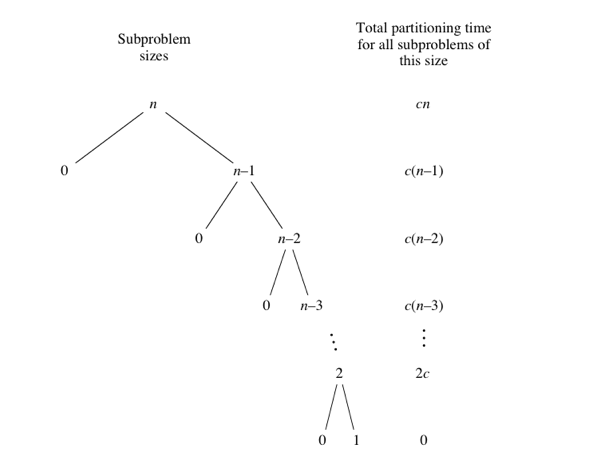
\includegraphics[scale=.5]{quicksort2}
\centering \linebreak \linebreak Figure: 
\end{figure}

When we add the times to do partitions for each level, we get as we have seen in other practices:\newline
\newline
$cn + c(n -1) + c(n -2) + ... + 2c = \sum_{j=1}^{i=-2} = \frac{(n-2)(n-1)}{2}$ \newline\newline
We can see that we have the arithmetic series, in notation big $\theta$, the complexity order is $\theta \in (n^{2})$\newline
\end{enumerate}

\pagebreak